	% IEEEtran V1.7 and later provides for these CLASSINPUT macros to allow the
	% user to reprogram some IEEEtran.cls defaults if needed. These settings
	% override the internal defaults of IEEEtran.cls regardless of which class
	% options are used. Do not use these unless you have good reason to do so as
	% they can result in nonIEEE compliant documents. User beware. ;)
	%
	%\newcommand{\CLASSINPUTbaselinestretch}{1.0} % baselinestretch
	%\newcommand{\CLASSINPUTinnersidemargin}{1in} % inner side margin
	%\newcommand{\CLASSINPUToutersidemargin}{1in} % outer side margin
	%\newcommand{\CLASSINPUTtoptextmargin}{1in}   % top text margin
	%\newcommand{\CLASSINPUTbottomtextmargin}{1in}% bottom text margin


	\documentclass[12pt,journal,compsoc]{IEEEtran}
	\usepackage[utf8]{inputenc}

	% *** CITATION PACKAGES ***
	\usepackage[nocompress]{cite}
	%\usepackage{cite}

	% *** GRAPHICS RELATED PACKAGES ***
	\usepackage[pdftex]{graphicx}
	\graphicspath{{img/}}
	\DeclareGraphicsExtensions{.pdf,.jpeg,.jpg,.png}

	% *** MATH PACKAGES ***
	\usepackage[cmex10]{amsmath}

	% *** SPECIALIZED LIST PACKAGES ***
	\usepackage[footnote]{acronym}
	\usepackage{algorithmic}

	% *** ALIGNMENT PACKAGES ***
	\usepackage{array}
	\usepackage{mdwmath}
	\usepackage{mdwtab}
	\usepackage{eqparbox}

	% *** SUBFIGURE PACKAGES ***
	\usepackage[caption=false,font=normalsize,labelfont=sf,textfont=sf]{subfig}
	%\usepackage[caption=false,font=footnotesize]{subfig}

	% *** FLOAT PACKAGES ***
	\usepackage{dblfloatfix}

	% *** PDF, URL AND HYPERLINK PACKAGES ***
	\usepackage{url}
	% Basically, \url{my_url_here}.


	% NOTE: PDF hyperlink and bookmark features are not required in IEEE
	%       papers and their use requires extra complexity and work.
	\newcommand\MYhyperrefoptions{bookmarks=true,bookmarksnumbered=true,
	pdfpagemode={UseOutlines},plainpages=false,pdfpagelabels=true,
	colorlinks=true,linkcolor={black},citecolor={black},urlcolor={black},
	pdftitle={Efficient 3D Isotropic Volume Reconstruction Based On 2D Tracked Ultrasound Images},
	pdfsubject={Introduction To Lab Research},
	pdfauthor={Keck Jean-Baptiste},
pdfkeywords={TIMC-IMAG, Introduction to Lab Research, Arthrosis, Ensimag, CUDA, GPGPU, Ultrasound Imaging, Isotropic Volume Reconstruction, Report}}
	

        \acrodef{gpgpu}[GPGPU]{General Purpose Computing on Graphics Processing Unit}
        \acrodef{cuda}[CUDA]{Compute Unified Device Architecture}
        \acrodef{timcimag}[TIMC-IMAG]{Techniques de l’Ingénierie Médicale et de la Complexité - Informatique, Mathématiques et Applications, Grenoble}
        \acrodef{gmcao}[GMCAO]{Gestes Médico-Chirurgicaux Assistés par Ordinateur}

	\begin{document}

	\title{Efficient 3D Isotropic Volume Reconstruction Based On 2D Tracked Ultrasound Images}

	\author{Jean-Baptiste Keck,~\IEEEmembership{Student,~Ensimag}\\
		Matthieu Chabanas,~\IEEEmembership{Supervisor,~TIMC-IMAG Laboratory}

	\IEEEcompsocitemizethanks{
	\IEEEcompsocthanksitem M. ~Keck is a student at Ensimag, Grenoble, France.
	\IEEEcompsocthanksitem M. ~Chabanas is in the team Gestes Médico-Chirurgicaux Assistés par Ordinateur in the TIMC-IMAG Laboratory, University of Grenoble, France. He was my supervisor for this project.}
	}


	% The paper headers
	\markboth{Introduction to Laboratory Research, Report,~Version.~1, No.~1, May~2014}
	{Shell \MakeLowercase{\textit{et al.}}: Bare Advanced Demo of IEEEtran.cls for Journals}
	%\IEEEspecialpapernotice{IRL Report}

\IEEEtitleabstractindextext{%
\begin{abstract}
	A miniature 3D tracked ultrasonic probe has been developped to aquire intra-articular cartilage images under artroscopic chirurgy conditions. The aim is to detect cartilaginous lesions (arthrosis) and quantize their precise sizes and locations to help the clinician in his diagnostic and his therapeutic decision making.
	The ultrasonic transducer is tracked by an optical locator, wich permits to find location and orientation of each 2D US images in a common 3D spacial reference. Near two thousands images are acquired when scanning a cartilage surface. An interesting tool is to rebuild a 3D isotropic volume (cubic voxels) with those images allowing further processing.
	Conventional 3D ultrasound algorithms have low computational complexity but the huge amount of data generated makes it difficult to compute results within reasonable time on classical computers. In this paper we investigate the possibilities of regenerating a 3D isotropic volume with the help of \ac{gpgpu} (\ac{cuda}) by adaptating existing algorithms to massive parallelism provided by modern everyday GPUs.
\end{abstract}

% Note that keywords are not normally used for peerreview papers.
\begin{IEEEkeywords}
	TIMC-IMAG, Introduction to Lab Research, Arthrosis, Ensimag, \acl{cuda}, \acl{gpgpu}, Ultrasound Imaging, Isotropic Volume Reconstruction, Report.
\end{IEEEkeywords}}


% make the title area
\maketitle

\section{Introduction}

\IEEEPARstart{T}{his} demo file is intended to serve as a ``starter file''
for IEEE Computer Society journal papers produced under \LaTeX\ using
IEEEtran.cls version 1.8 and later.
I wish you the best of success \cite{1}.

\hfill mds
 
\hfill December 27, 2012

\subsection{Subsection Heading Here}
Subsection text here.

% needed in second column of first page if using \IEEEpubid
%\IEEEpubidadjcol

\subsubsection{Subsubsection Heading Here}
Subsubsection text here.


\begin{figure}[!t]
\centering
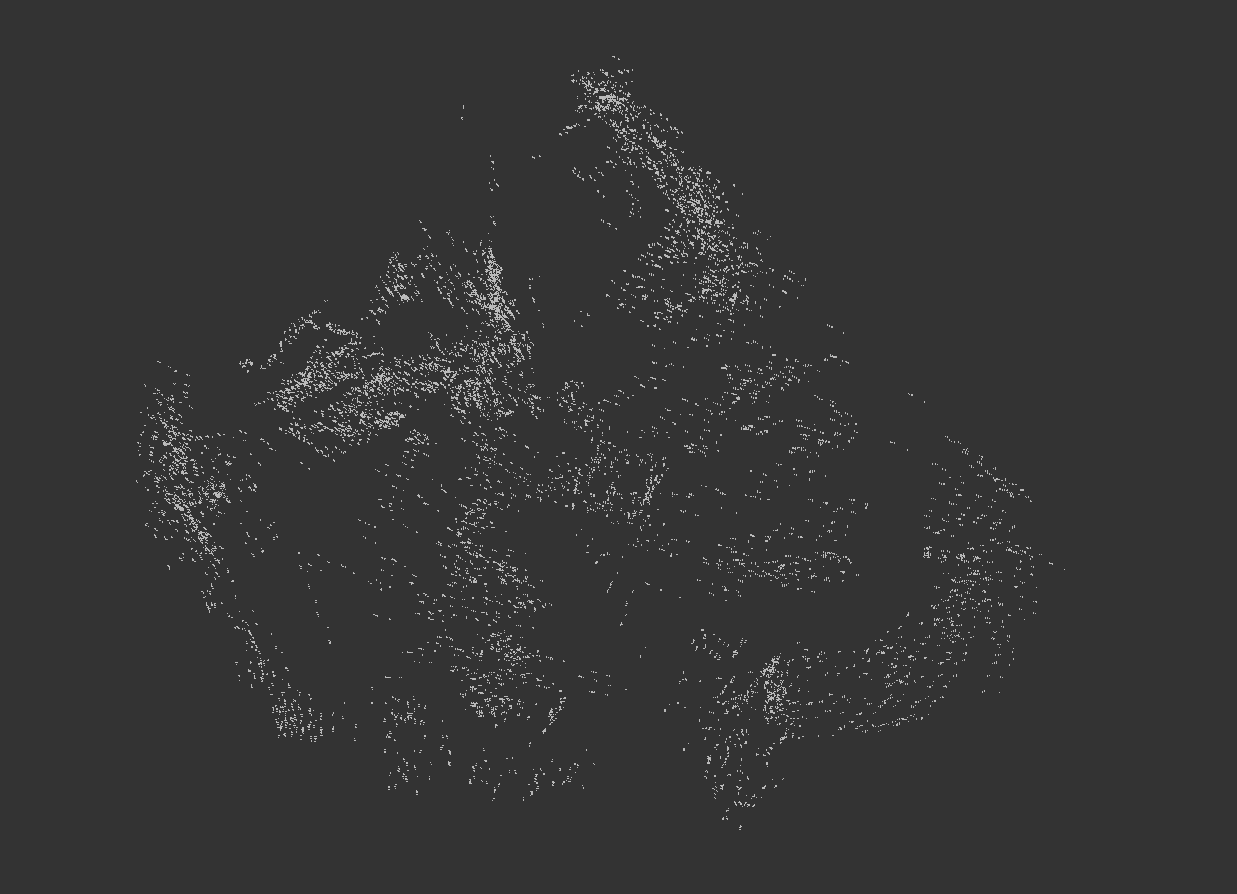
\includegraphics[width=2.5in]{femur_2}
\caption{Simulation Results.}
\label{fig_sim}
\end{figure}

\begin{figure*}[!t]
\centering
\subfloat[Case I]{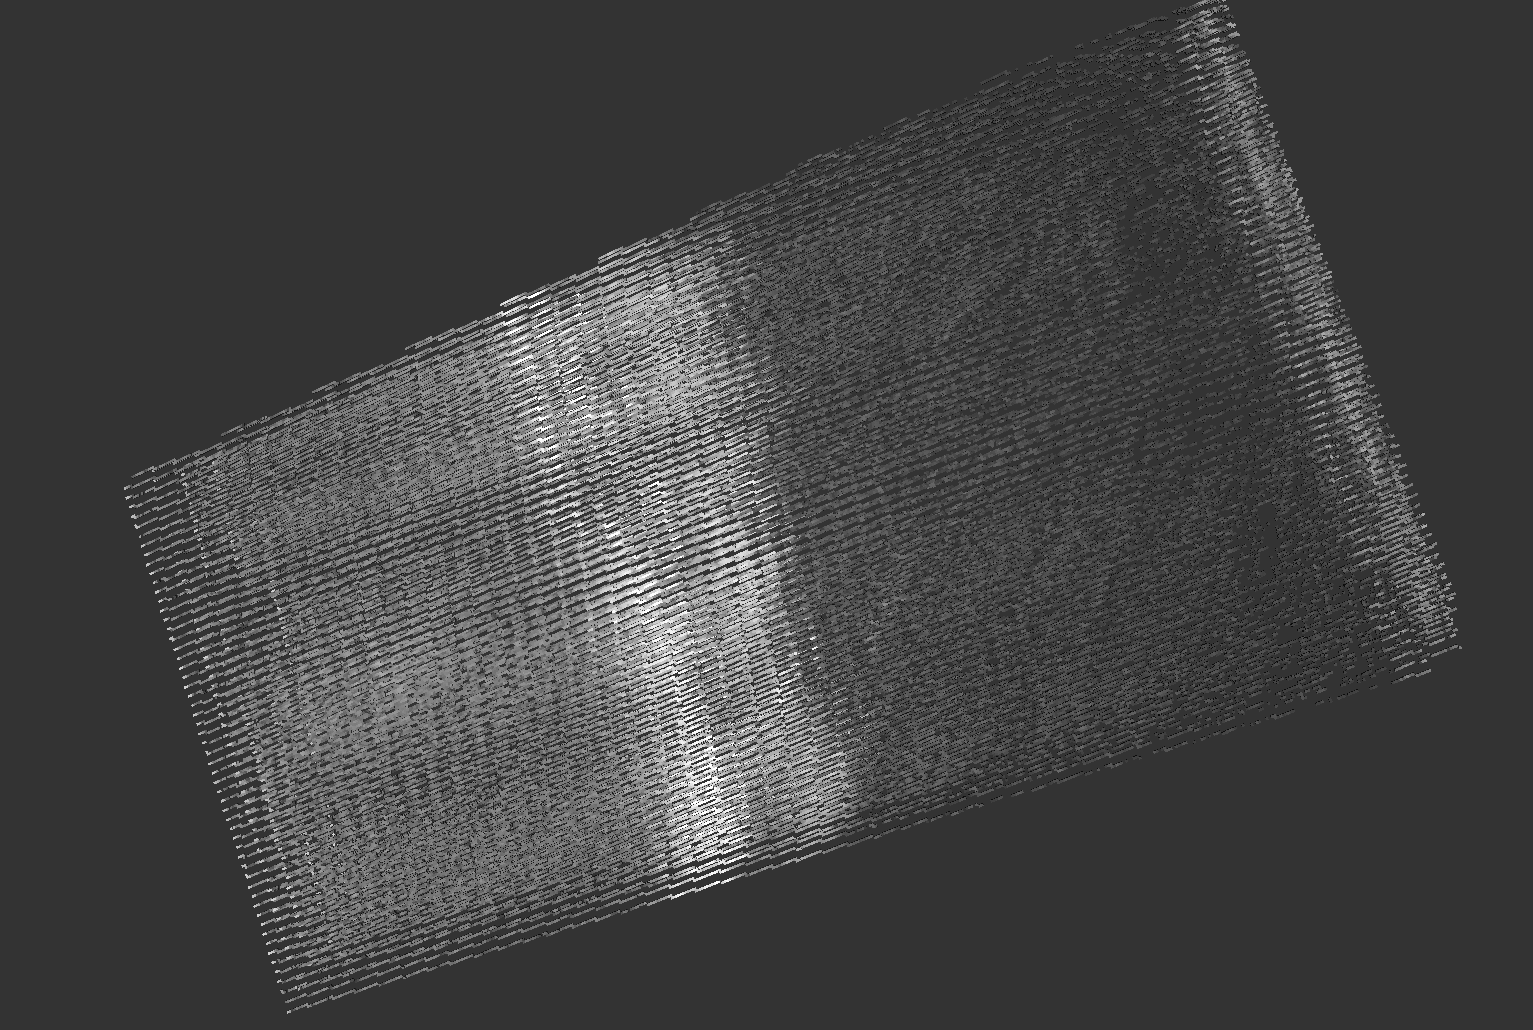
\includegraphics[width=1.5in]{data_0}%
\label{fig_first_case}}
\hfil
\subfloat[Case II]{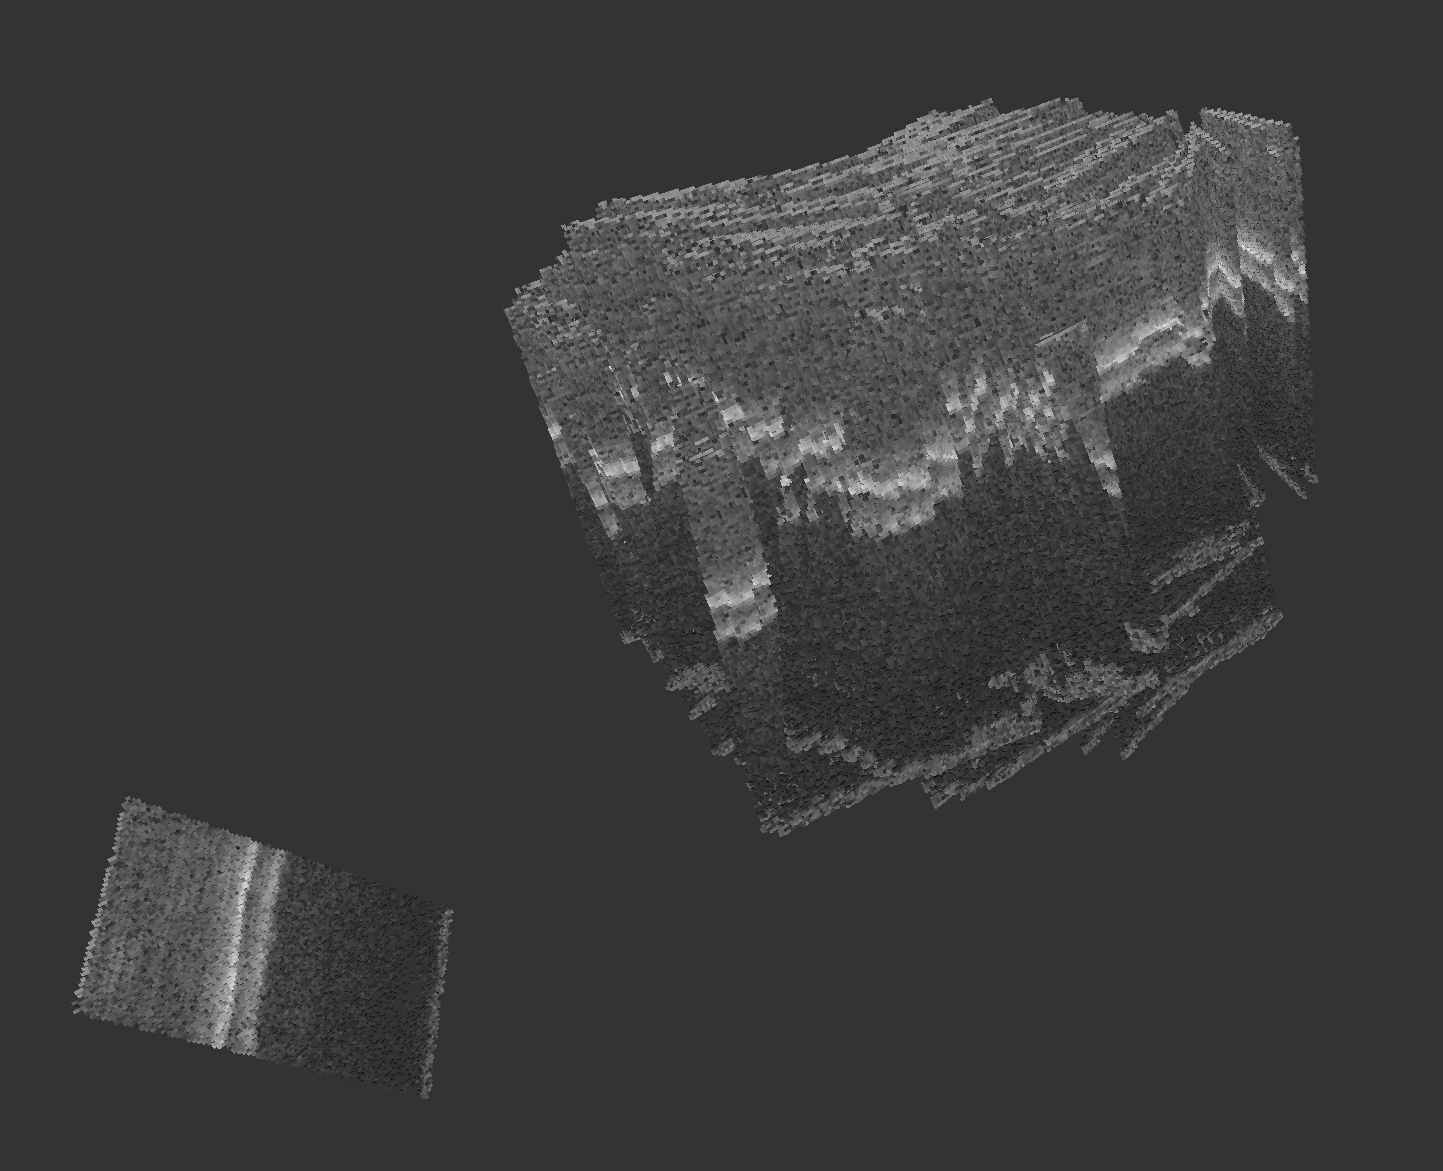
\includegraphics[width=1.5in]{data_1}%
\label{fig_second_case}}
\hfil
\subfloat[Case III]{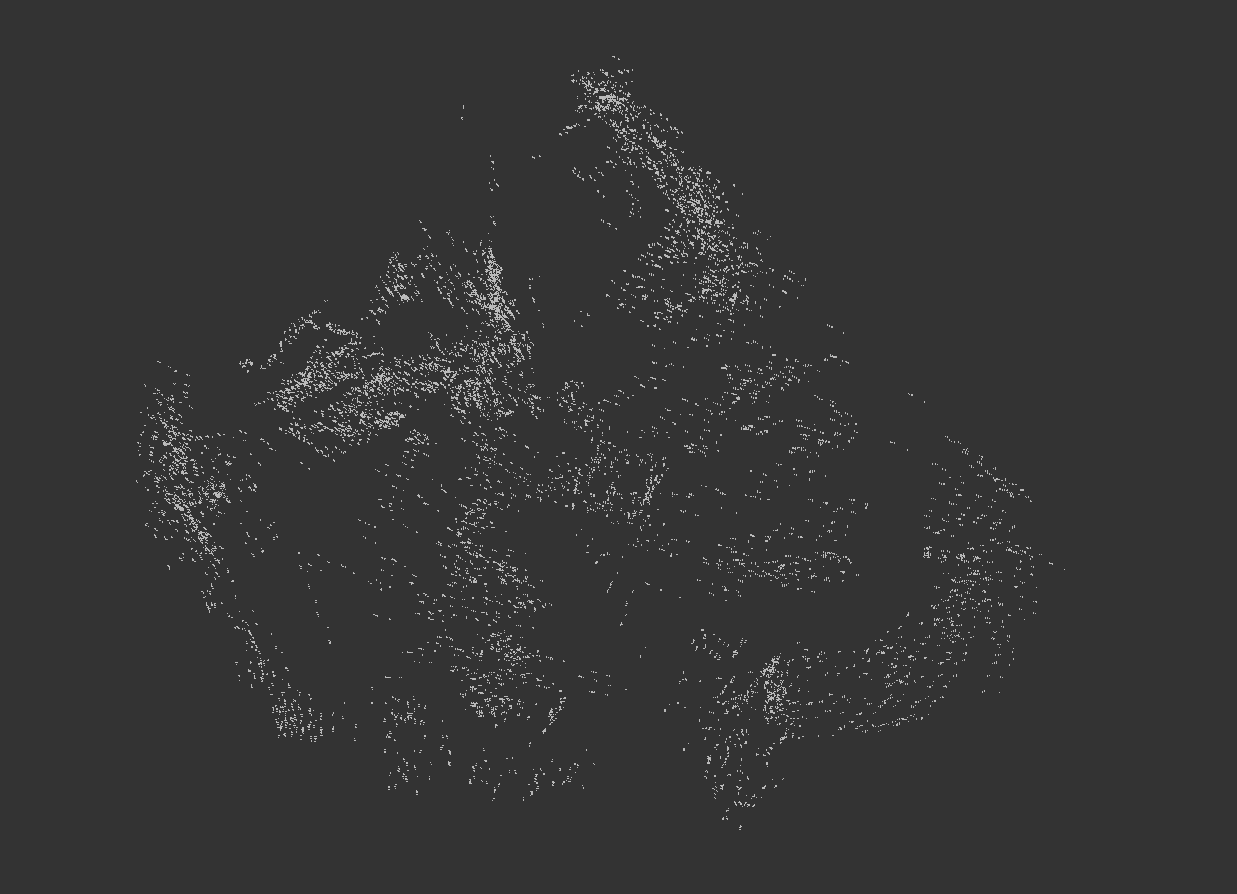
\includegraphics[width=1.5in]{femur_2}%
\label{fig_third_case}}
\caption{Simulation results.}
\label{fig_sim}
\end{figure*}
%
% Note that often IEEE papers with subfigures do not employ subfigure
% captions (using the optional argument to \subfloat[]), but instead will
% reference/describe all of them (a), (b), etc., within the main caption.

% An example of a floating table. Note that, for IEEE style tables, the 
% \caption command should come BEFORE the table. Table text will default to
% \footnotesize as IEEE normally uses this smaller font for tables.
% The \label must come after \caption as always.

\begin{table}[!t]
% increase table row spacing, adjust to taste
\renewcommand{\arraystretch}{1.3}
%if using array.sty, it might be a good idea to tweak the value of
%\extrarowheight as needed to properly center the text within the cells
\caption{An Example of a Table}
\label{table_example}
\centering
% Some packages, such as MDW tools, offer better commands for making tables
% than the plain LaTeX2e tabular which is used here.
\begin{tabular}{|c||c|}
\hline
One & Two\\
\hline
Three & Four\\
\hline
\end{tabular}
\end{table}



\section{Conclusion}
The conclusion goes here.



\appendices
\section{Images Coordinate System}
appendix text goes here.

\section{Existing Algorithms}
appendix text goes here.

% you can choose not to have a title for an appendix
% if you want by leaving the argument blank
\section{Voxel Renderer}
Appendix text goes here.

\section*{Acknowledgments}
I would like to thank the TIMC-IMAG laboratory for having hosted me for 4 months, especially the GMCAO team members that were always here to help when there were any problems and for the good mood. Special thanks goes to M. Chabanas for having taken the time and energy throughout the project by providing precious feedbacks and for having introduced me to the TIMC-IMAG laboratory.

% Can use something like this to put references on a page
% by themselves when using endfloat and the captionsoff option.
\ifCLASSOPTIONcaptionsoff
  \newpage
\fi


\bibliographystyle{IEEEtran}
\bibliography{master}


% biography section
% 
% If you have an EPS/PDF photo (graphicx package needed) extra braces are
% needed around the contents of the optional argument to biography to prevent
% the LaTeX parser from getting confused when it sees the complicated
% \includegraphics command within an optional argument. (You could create
% your own custom macro containing the \includegraphics command to make things
% simpler here.)
%\begin{IEEEbiography}[{\includegraphics[width=1in,height=1.25in,clip,keepaspectratio]{mshell}}]{Michael Shell}
% or if you just want to reserve a space for a photo:

\begin{IEEEbiography}{Michael Shell}
Biography text here.
\end{IEEEbiography}

% if you will not have a photo at all:
\begin{IEEEbiographynophoto}{John Doe}
Biography text here.
\end{IEEEbiographynophoto}

% insert where needed to balance the two columns on the last page with
% biographies
%\newpage

\begin{IEEEbiographynophoto}{Jane Doe}
Biography text here.
\end{IEEEbiographynophoto}

% You can push biographies down or up by placing
% a \vfill before or after them. The appropriate
% use of \vfill depends on what kind of text is
% on the last page and whether or not the columns
% are being equalized.

%\vfill

% Can be used to pull up biographies so that the bottom of the last one
% is flush with the other column.
%\enlargethispage{-5in}

\end{document}
